\documentclass[10pt,twocolumn,letterpaper]{article}

\usepackage{cvpr}
\usepackage{times}
\usepackage{epsfig}
\usepackage{graphicx}
\usepackage{amsmath}
\usepackage{amssymb}

% Include other packages here, before hyperref.

% If you comment hyperref and then uncomment it, you should delete
% egpaper.aux before re-running latex.  (Or just hit 'q' on the first latex
% run, let it finish, and you should be clear).
\usepackage[breaklinks=true,bookmarks=false]{hyperref}

\cvprfinalcopy % *** Uncomment this line for the final submission

\def\cvprPaperID{****} % *** Enter the CVPR Paper ID here
\def\httilde{\mbox{\tt\raisebox{-.5ex}{\symbol{126}}}}

% Pages are numbered in submission mode, and unnumbered in camera-ready
%\ifcvprfinal\pagestyle{empty}\fi
\setcounter{page}{1}
\begin{document}

%%%%%%%%% TITLE
\title{Optical Character Recognition of Japanese Text}

\author{Chase Basich\\
Stanford University\\
{\tt\small cdbasich@stanford.edu}
% For a paper whose authors are all at the same institution,
% omit the following lines up until the closing ``}''.
% Additional authors and addresses can be added with ``\and'',
% just like the second author.
% To save space, use either the email address or home page, not both
\and
Sloane Sturzenegger\\
Stanford University\\
{\tt\small sloanes@stanford.edu}
}

\maketitle
%\thispagestyle{empty}

%%%%%%%%% ABSTRACT
\begin{abstract}
Japanese Optical Character Recognition is still a developing field. Standard methods developed for the Latin alphabet do not perform well with Japanese, due to Japanese having many more characters: about 2,800 common characters out of a total set of more than 50,000. Each Japanese character is, on average, more complicated than an English letter. This paper introduces a character recognition system for Japanese combining standard image segmentation and classification techniques with large, state-of-the-art feature sets. Our system performs well across two tests, one that validates the algorithm’s success at identifying high quality images of characters in a variety of fonts and an experiment in extracting characters from a raw scan of a Japanese document.

The system developed in this paper uses advanced feature representations and provides excellent results, despite having an extremely limited number of training points for each character. We believe that this system will only improve with more data points and is capable of recognizing both typeset and handwritten characters across many Asian languages beyond just Japanese.
\end{abstract}

%%%%%%%%% BODY TEXT
\section{Introduction}
Provide a concise statement of the problem you’re tackling and the solution you’re implementing. Discuss the scope of the technical work (sub component development vs. exhaustive experimental validation of existing algorithms). Discuss how it relates to the literature. Provide a brief outline of the paper’s content and sections.

We have developed a software system for recognizing Japanese characters from images. The challenge of Japanese OCR is in its huge number of characters. The sheer number of characters hints at the fact that each Japanese character is, by definition, much more complex than an English character. There are three different alphabets in Japanese, but for this problem, we can treat all characters as members of the same superset. The ultimate goal of any OCR system is to recognize handwritten characters. Training a recognizer across some 2,000 different classes is an extremely daunting challenge and requires significant feature engineering to create a large enough feature space to isolate a character.

Even for one character, there is a significant amount of variation between fonts, just like English. These types are differences are accentuated by the larger number of strokes per character. Consider the character 穫 (meaning ‘to harvest’) in several of the fonts used in our training set. In some fonts, the strokes connect, but in others, they do not. These changes exaggerate the ambiguity within characters and make classification especially difficult.

\begin{figure}[t]
    \centering
    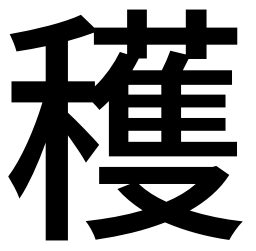
\includegraphics[width=0.4\columnwidth]{../data/kanji-Boku2/kanji_225.png}
    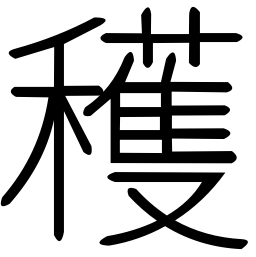
\includegraphics[width=0.4\columnwidth]{../data/kanji-Chigfont/kanji_225.png}
    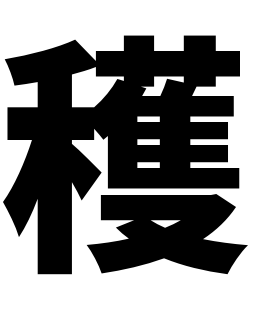
\includegraphics[width=0.4\columnwidth]{../data/kanji-GenEiHeavy/kanji_225.png}
    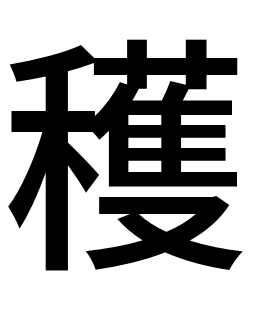
\includegraphics[width=0.4\columnwidth]{../data/kanji-GenEiSemiBold/kanji_225.png}
    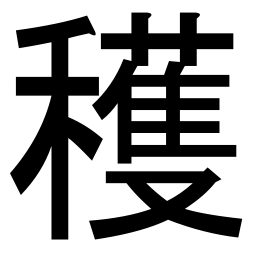
\includegraphics[width=0.4\columnwidth]{../data/kanji-Gothic/kanji_225.png}
    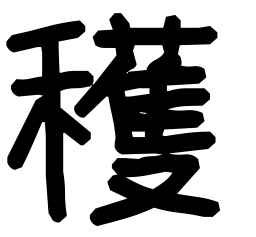
\includegraphics[width=0.4\columnwidth]{../data/kanji-HonyaJi/kanji_225.png}
    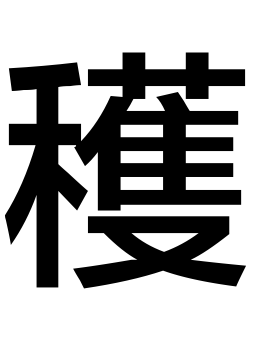
\includegraphics[width=0.4\columnwidth]{../data/kanji-Lantinghei/kanji_225.png}
    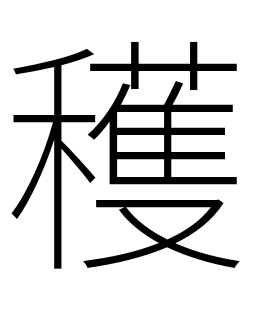
\includegraphics[width=0.4\columnwidth]{../data/kanji-GenEiExtraLight/kanji_225.png}
    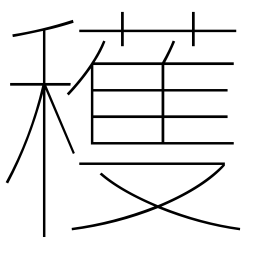
\includegraphics[width=0.4\columnwidth]{../data/kanji-Chogokubo/kanji_225.png}
    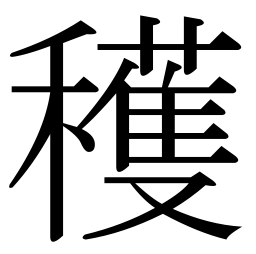
\includegraphics[width=0.4\columnwidth]{../data/kanji-Mincho/kanji_225.png}
    \caption{The character for ``to harvest'' across many fonts.}
\end{figure}

For those unfamiliar with the Japanese language and its textual structure, each character is called a kanji. Kanji themselves are made up of bushu (called “radicals” in English) and a word is made of potentially multiple kanji. There are no spaces in Japanese to separate words. The process of splitting Japanese characters into words remains an unsolved problem and is outside the realm of this class.

Our solution has a two-phase approach. The first step of is image segmentation. Our segmentation in well-formed documents is fairly simple, where we use a simple heuristic, which is sufficient for the task of extraction of text that is typewritten and scanned. An interesting area of future work will be the extract of text from non-document images, like road signs, colorful menus, or even sports jerseys. Once we’ve segmented one character from the image, we can use our feature extractor and a Naive Bayes predictor to identify the character. We have a large feature space, which is a necessity to distinguish across the few thousand different characters. The most important contribution of this paper is its implementation and discussion of features and how they affect the success of a machine learning classifier. The classifier presented here outperforms a commercial, online Japanese OCR tool for certain fonts and we believe it would outperform it on all fonts, given enough training data.

\section{Previous Work}
There is a surprisingly small amount of literature in English focusing specifically on on Japanese OCR methods. More research exists in Chinese fonts, but given that the two languages share many characters, we believe that the lessons from one language can be shared with the other. In fact, the alphabets of several east Asian languages (these two and also Korean and Vietnamese) stem originally from the Chinese language.

One invaluable resource was Fumitaka Kimura’s paper OCR Technologies for Machine Printed and Hand Printed Japanese Text. This paper provides a broad survey of available preprocessing and feature-extraction techniques that are used in modern systems. Kimura introduces several important preprocessing steps that we leverage in our system. Kimura provides the reasoning and mathematical basis for skew-correction and outlines a simplistic algorithm for line and character segmentation within well-formed documents. The algorithm Kimura introduces takes advantage of Japanese being fixed pitch -- almost every character in Japanese is roughly the same size, as compared to English, where a lowercase i is much narrower than an uppercase W. Kimura also suggests an advanced skewing operation as a preprocessing step before extracting features. Japanese characters are more dense in the center than they are at the edges. He applies a transformation akin to a fisheye lense: expand the center of the image while decreasing the size of the edges.

One of the most important features that increases accuracy for Chinese OCR comes from Xianli Wu and Min Wu and their paper A Recognition Algorithm For Chinese Characters In Diverse Fonts. In the paper, they introduce a new feature called peripheral directional contributivity. Its implementation is detailed below in SECTION SECTIONNUMBER. This was the most powerful feature we found during our research. The Wu and Wu paper trains different classifiers for each font using the PDC feature. They then train and test on the same font, which delivers excellent results -- averaging 98.6\% accuracy across a test corpus of eight font faces. While impressive, their algorithm is not tested on unseen fonts, which limits its applicability to documents in general. We attempt to improve upon their work by training one classifier across all fonts, which eliminates the need to know the font ahead of time.

\section{Technical Solution}
The problem reduces to three sub-problems. First, we need to identify where in an image kanji appear and separate those kanji into individual subimages. Next, we need to classify that character by extracting its important features. However, this is true of all OCR systems, not just Japanese. What makes Japanese OCR more difficult is the large number of characters, as explained in the introduction. This forces us to use a much broader selection of features, not to mention using a larger quantity of them as well.

The approach outlined below is implemented in Python using OpenCV as its image processing library, SciPy and NumPy for sophisticated mathematical processing, and the scikit-learn package for machine learning. By leveraging a user-friendly language that easily calls into C and C++ functions, our solution is reasonably efficient while also allowing for rapid development.


\subsection{Segmentation}
The heuristic used in image segmentation assumes that lines of text are all oriented in the same direction. Furthermore, it relies on the text being fixed-pitch, meaning that each character is given close to the same space regardless of the size of the character itself. Segmentation is performed on a binary version of the image: pixel values over the threshold are black and those under the threshold are white.

The segmentation process occurs in three steps. First, the orientation of the image must be normalized so the kanji are not rotated and each line of characters is strictly horizontal. This is achieved by searching for the orientation that maximizes the horizontal whitespace between each line of text.  After the orientation is determined, an assumption is made that there is whitespace between each line of text and that all lines are oriented the same direction. The image is then cut into lines delimited by whitespace in the vertical direction.

Finally, each line is processed so each character is segmented so it can be classified with the minimum amount of noise. To do this, we first need to estimate the pitch of the line, as for a given line, each character is given approximately the same amount of horizontal space, regardless of the width of the character itself. To estimate, we find the width of all characters in the line which are horizontally contiguous and do not have white space separating two halves of the character, discard the outliers, and then average the width of the remaining characters. To then segment the line into characters, we find the column of pixel values with the least black pixels closest to the estimated cutting point determined by the pitch of the line.

\begin{figure}[t]
    \centering
    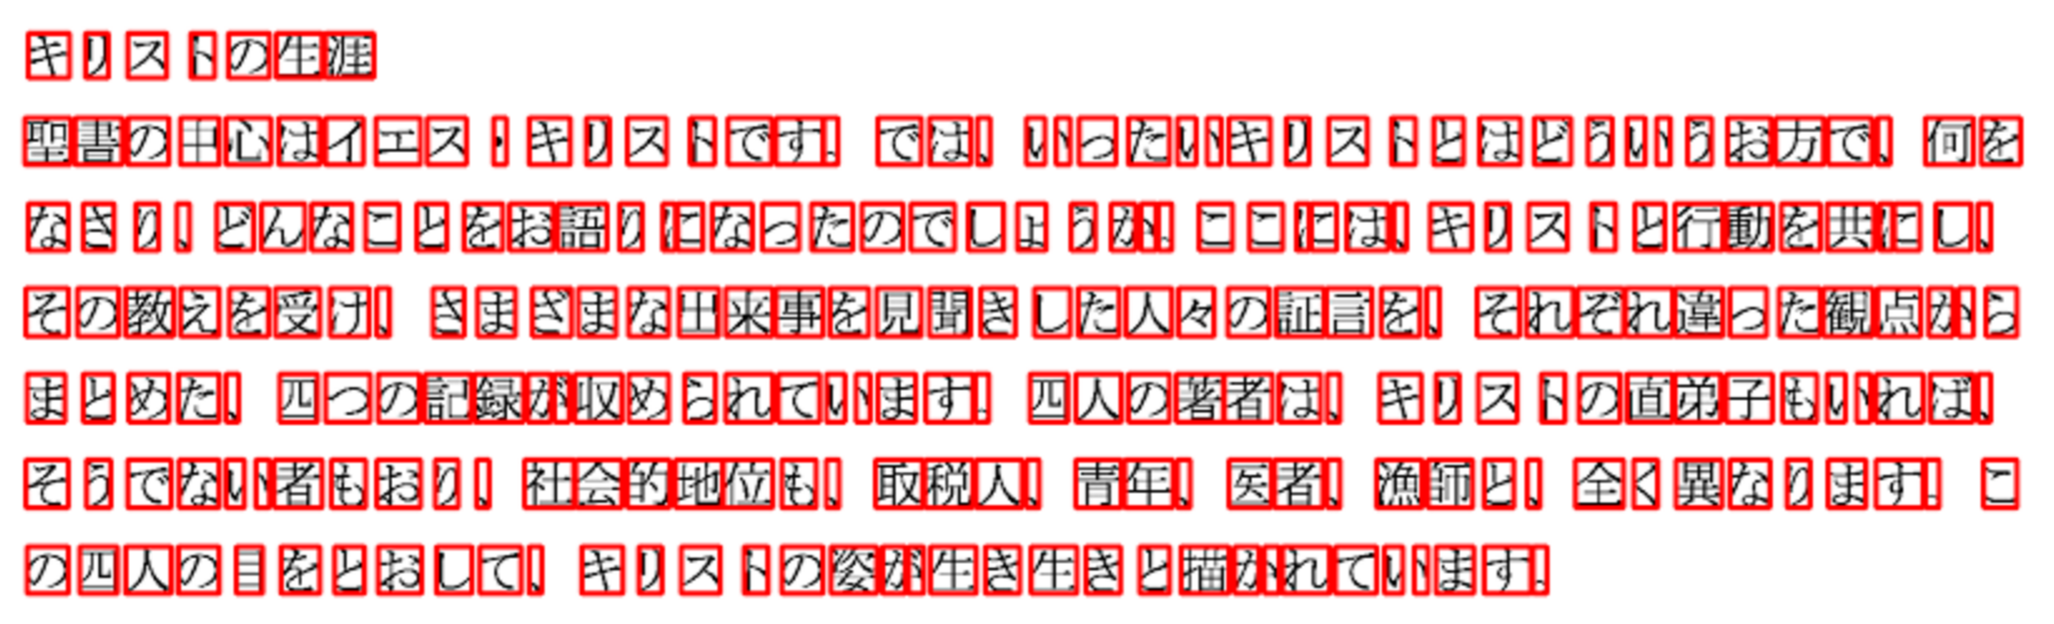
\includegraphics[width=\columnwidth]{../segmented.png}
    \caption{Example of segmented kanji.}
\end{figure}

\subsection{Classification}
Classification is the process where the candidate image is compared against historically observed golden image-kanji pairs in order to select a most likely kanji for the image in question. Small candidate kanji images are cropped out of the original document’s image by the segmentation engine and flow into the classifier.

The classifier has two distinct stages: first the training step and then the classification stage. The system uses a classic machine learning method: Gaussian Naive Bayes. In developing this report, we experimented with several underlying machine learning algorithms but settled on Naive Bayes when it provided the best results on our test data.

In order to provide robust prediction across the many thousands of characters, the system needs a very large feature space. In order to provide such a large feature space, there are several different classes of features used, which are all concatenated into one long vector for the Naive Bayes training and classification procedures. A significant portion of this project is based around excellent feature engineering, so included is a description of each feature vector that is included as a part of the entire feature vector.

\subsubsection{Preprocessing}
Before entering the machine learning pipeline, all images undergo a series of transformations in order to standardize the input images across different fonts and documents. First, we convert all images to binary, making the darkest pixels the foreground main font and the background standard white pixels. Then, all the whitespace around the edge of the image is cropped away, finding the tightest bounding box possible for the character. This prevents the effects of varying segmentation from causing irregularities when we extract features. Finally, for some features, we normalize the image into a 48-by-48 square. Normalizing to a small square helps to accentuate the fundamental aspects of the image and limit the effects that the font artist’s creativity can overwhelm our features.

\subsubsection{Peripheral Direction Contributivity}
The most important and distinctive feature included in the system is the PDC feature which was invented by Xianli Wu and Min Wu in their paper for IEEE ICIP ‘02  [CITATION NEEDED]. The PDC feature vector was designed to recognize Chinese characters across a diverse group of fonts but generalizes quite well to Japanese, whose alphabet shares many characters with that of Chinese.

As an introduction, it is important to realize that in Japanese characters, the strokes  occur primarily in the cardinal directions and along the diagonals. Features should try to capture, in the smallest vector possible, the number of strokes, the orientation of strokes, the location of the strokes, and the length of the strokes. Implicit in those features is also the intersection of the strokes in a character. Each character is fundamentally defined by these types of parameters.

The PDC feature vector attempts to capture these features by first reducing each image to a 48 x 48 pixel square. In this representation, a stroke can be anywhere from 1 to 5 pixels in width and can be up to 30 or 40 pixels long. PDC searches through the image in all directions to identify the length of strokes in that direction.

A PDC feature vector is built in the following way. After scaling the image down or up, the program looks at each row. For each row, the program scans across each row from left to right and counts how many consecutive black pixels are observed in each grouping of black pixels in that row. The length of the first three black groupings is recorded. The process is repeated for all rows, columns, and diagonals in eight different directions: the compass directions and all 45-degree angles. The sixty-four three-tuples recorded for each row or column (127 three-tuples for the diagonals) are averaged into overlapping groups of four. Figure FIGNUM1 (from the Wu and Wu paper) demonstrates how pixels are counted along the eastern direction and it is easy to identify the three clusters of black pixels in that row.

\begin{figure}[t]
    \centering
    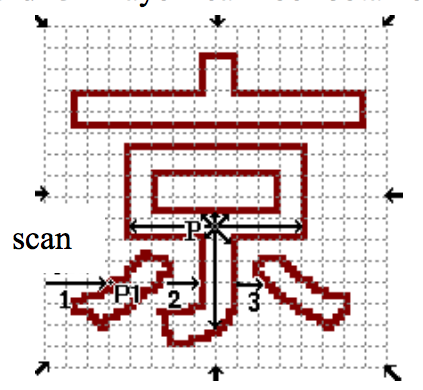
\includegraphics[width=0.7\columnwidth]{../pdc.png}
    \caption{Construction of PDC feature vector.}
\end{figure}


\subsubsection{ORB Features}
Another important feature leveraged in the system is the ORB feature, short for Oriented FAST and Rotated BRIEF). It is extremely similar to the SIFT system and was invented by the Willow Garage robot research lab. The authors of the algorithm argue that it is an efficient alternative to SIFT or SURF. Japanese characters are frequently written at a slant that can vary between authors (in handwritten text) or between fonts (in typeset documents). By using a very efficient system that compares favorably to a rotation-invariant version of both FAST and BRIEF, our system gains more insight into the fundamental keypoints of a given japanese character representation. ORB is implemented in OpenCV already, so we simply integrate it into the system.

The two similar feature systems that ORB aims to reproduce are FAST and BRIEF. FAST is a corner-detection algorithm that uses gradients to efficiently find locations where a sharp change in color forms a roughly concave shape. BRIEF is based around a binary descriptor and also aims to identify key points that fundamentally distinguish one image from another.

\begin{figure}[t]
    \centering
    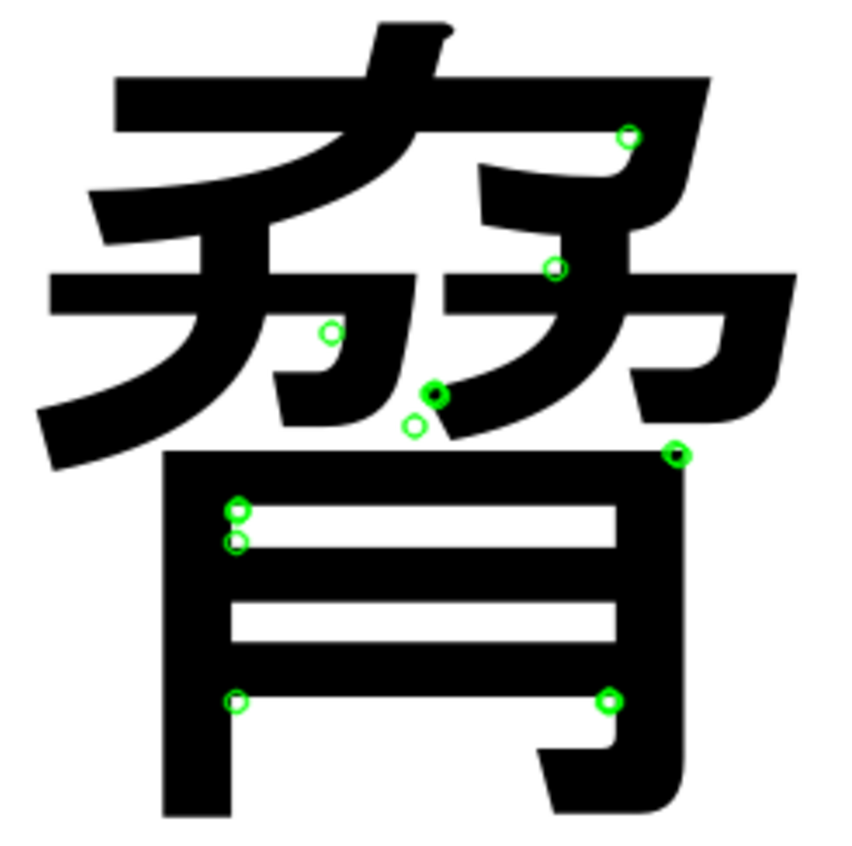
\includegraphics[width=0.7\columnwidth]{../orb.png}
    \caption{ORB keypoints for a kanji.}
\end{figure}

\subsubsection{Histogram of Oriented Gradients}

Another significant feature is the histogram of oriented gradients, which was used in CS231A earlier this quarter. As a refresher, the HoG feature works by computing a dense grid of uniform cells to find the direction and magnitude of gradients per pixel. It then bins these gradients into a histogram and uses a rolling, overlapping average to compute a histogram for each section of the image. Adding the HoG gradient helps the machine learning algorithm gain a sense of the edges and borders of an image. This is a great boon to our system, as the edge positions of a Japanese character are an excellent correspondence between two images of the same character in different fonts.

Although a form of HoG is implemented in OpenCV, we re-implemented the HoG algorithm to get further control of the histogram bin size and other hyperparameters. Adding in the HoG vector to our overall feature vector was extremely important in boosting the performance of the system.

\subsubsection{Center of Gravity}

An important aspect to consider when looking at Japanese characters is the amount of pixels distributed through different parts of the image. Some kanji have extremely dense regions and other non-dense regions. In order to capture that, we calculate the pixel center of gravity for each quadrant of the image, in addition to the overall center of gravity for the character. The center of gravity is also called the center of mass and is calculated by scipy using the location of each black pixel in the quadrant. This feature was inspired by Yichang Shi and Donglai Wei who have researched OCR in Sanskrit and cite the center of gravity as an important feature in their research.

\begin{figure}[t]
    \centering
    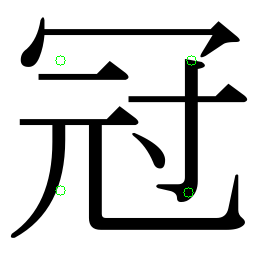
\includegraphics[width=0.7\columnwidth]{../cog.png}
    \caption{The center of gravity for the 4 quadrants of this character.}
\end{figure}

\subsubsection{Global Features}

A last feature vector we implemented was also suggested by Shi and Wei’s work on Sanskrit. We have a few features that look “globally” at the image, rather than splitting it up into pieces to calculate a pixel-by-pixel factor like HoG or PDC. This feature does not use the resized image, but rather the original kanji extracted from the segment step. Each global feature is a simple calculation that looks at the entire image, rather than scanning across in bins like histograms of oriented gradients or in rows like the peripheral directional contributivity.

\begin{itemize}
    \item The height-to-width ratio of the image image. This helps to distinguish tall and skinny kanji from short and fat characters.
    \item The center of mass across the entire image in the x-direction. The center of mass along the x-axis separates left-heavy from right-heavy kanji.
    \item The center of mass across the entire image in the y-direction. Just like it’s x-axis sibling, this distinguishes top-heavy from bottom-heavy characters in the dataset.
    \item The standard of deviation in black pixels across the x-direction. The standard of deviation helps to illustrate how tightly pixels are clumped in one section, potentially representing the number of bushu in the kanji.
    \item The standard of deviation in black pixels across the y-direction. This is justified the same as the x-axis standard of deviation feature. The larger the standard of deviation, the more evenly spread the kanji is across its entire width.
    \item The ratio of filled to empty pixels across the entire image. This is an important feature that serves as a rough proxy for how many strokes are in the image.
\end{itemize}

\section{Experimental Setup \& Results}
\subsection{Setup}
We have two experiments: testing well-formed, identically generated images of each character from each font, and testing our system in parsing an actual document. The two tests have the first half of the setup in common, they both are trained from the same training data.

To generate the training data, for each font we generate a png file for each character in the hiragana alphabet, the katakana alphabet, and the Joyo subsection of Kanji. These kanji are the 2,136 characters recognized by the Japanese government as the most important kanji and the only kanji that are permitted for use in official government documents. Each character has an image generated in each of the 21 fonts.

\subsection{Experiment 1}
In this experiment, we train our Gaussian Naive Bayes classifier over 20 of the 21 fonts and test each character from the remaining font. We’ve subdivided our list of fonts into four categories called  “Standard”, “Thick”, “Thin”, and “Serifed”. To better understand the performance of our system and the efficacy of our feature selection, we tested one font from each category against the remaining 20 fonts.

\begin{table}
    \centering
    \begin{tabular}{|c|c|c|c|}
        \hline
        Standard & Thick & Thin & Serif \\
        \hline
        93.2\% & 80.5\% & 84.\% & 35.0\%\\
        \hline
    \end{tabular}
    \caption{The performance of the classifier in Experiment 1.}
\end{table}

\subsection{Experiment 2}
This experiment tests both our image segmentation and subsequent classification of segmented kanji. We were unable to obtain a corpus of original handwritten Japanese text or the digital transcriptions of text in images, as the only one available in the US were prohibitively expensive and corpuses from Japan would not have arrived here in time, as they would have been physically shipped and could not be transferred digitally. Our criteria then shifted to easily accessible, open source, and with a wide range of characters. The first thing we found which fit this criteria was the Bible, so we chose to test our system on images of pages from the new Testament Book of Matthew.

For each page in Matthew, our system first segments in the image into individual characters and then classifies it using the classification system described above. After collecting the output in a text file, we evaluate the success by measuring the Levenshtein edit distance from the original file. Edit distance is a measurement of how different two pieces of text are, with a penalty for each missing, added, or incorrect character.

To establish meaningful baseline results, we similarly test against i2OCR.com, the only free online Japanese OCR tool we found to perform with a significant degree of correctness (we tested other systems online and they all failed to correctly classify a single character in the image). We consider this the silver standard against which we can compare our results: if our OCR tool works better than this website, we consider it a success.

As a third measurement, we also test the image classification after only training on the font used in the version of Matthew. The purpose of this test is to determine the degree of overfitting in our features and how effectively the classification engine is when considering a smaller version of the same image (our training images are about 256 pixels square, whereas the segmented images from the Bible are about 75 pixels square, losing a lot of their detail).

\begin{table}
    \centering
    \begin{tabular}{|c|c|c|}
        \hline
        Training all fonts & Training one font & i2OCR.com \\
        \hline
        703 & 199 & 502 \\
        \hline
    \end{tabular}
    \caption{Levenshtein edit distance when testing a serif font.}
\end{table}

\begin{table}
    \centering
    \begin{tabular}{|c|c|c|}
        \hline
        Training all fonts & Training one font & i2OCR.com \\
        \hline
        703 & 199 & 502 \\
        \hline
    \end{tabular}
    \caption{Levenshtein edit distance when testing a sans-serif font.}
\end{table}

\subsection{Discussion: Segmentation}
The segmentation used in this project worked very well and was not a major contributing source of error. It was able to successfully handle the cases where the character had a wide horizontal gap in the middle, which a more standard segmentation system would treat as separate characters.

\subsection{Discussion: Serif vs. Sans-Serif}
Even late into the project, it was not obvious that the type of font mattered nor that the fonts could be divided into obvious styles like serif and sans-serif. However, upon inspection of our data, we realized this distinction had many important implications.

In Experiment 1, the reasons for the discrepancy between serif fonts and sans-serif fonts is quite clear, we not only have fewer serif fonts than sans-serif fonts, but each serif font has a unique style of serifs that provide more distinct features than each sans-serif font. Each sans-serif font is very similar to its san-serif cohort, which is not true for serif fonts.

Our understanding of and explanation for the results in Experiment 2 is more nuanced and far less obvious.

First, when only training on one image, we argue that for the sans-serif font the system can find very few distinguishing features for each character and overfits the data on the exact training examples its sees. However, serif fonts are more ornate and have more complex structure, which offers more details for the classifier to grasp ahold to. When tested against scaled-down versions of the same font, the ambiguity of the sans-serif font is accentuated and the overfitting severely degrades the performance, while the serif font still has enough good features to be fairly accurate.

When training with all of the available fonts, the performance improves for sans-serif and declines for serif fonts. This is because the large number of sans-serif fonts helps the classifier reduce overfitting and understand exactly what makes up a character in its sans-serif representation. At the same time, however, we lose track of what the serif fonts look like: a leading factor causing this is most likely our dearth of training serif fonts. The tested serif font, with its more decorative flair, causes confusion for the classifier and ultimately poor performance. Our belief is that this is due to characters in serif fonts having more distinguishing features. Said more simply, two characters in a sarif font will appear less similar than in a sans-serif font. The lack of good training data is a major factor in both Experiment 1 and Experiment 2.

\section{Future Work}

\subsection{Selecting Training Data}
Our first conclusion is very obvious: we need more fonts. It is clear that training on such a limited set of fonts leads to overfitting of training data and an unreliable classifier. However, this might not be a feasible solution: there simply are not many fonts for Japanese characters. We instead examine other possible solutions in light of our results.

Instead of training on all fonts, our data suggests that a reasonable approach would be to first determine whether a serif font or a sans-serif font is present in the document. We can see that by selectively training over the proper class of font can result far fewer errors. This step is reflected in previous research, where training was always performed over same font that is used in testing. [CITATION OF WU AND WU]

\subsection{Selecting Features}
Given that we are only working with machine-printed images that are normalized to 48x48 pixels, we did not expecting overfitting to be a large source of error. However, our results show that the features present in an image that has been normalized from 300x300 a pixel image differ significantly from those present in an image that is generated at 48x48 pixels. Future work should identify which features are more critical given the size of the training set.


\subsection{Handwriting}

OCR on Japanese handwriting is an ongoing research problem and we will briefly discuss some of the challenges in implementing such a system, in light of our results.

The first major issue is the lack of accessible, sizeable training corpuses. Even when working with typeset fonts, we can see that a large training set is required to prevent overfitting. As handwriting has more variation than typed fonts, this issue is compounded. However, there has not been a major attempt to create large corpuses of handwriting in Japanese.

The next issue is that our system in particular is not extendable to Japanese handwriting. Our feature selection process requires strokes with widths of greater than 1 pixel and which are oriented along the cardinal directions and the major diagonals. However, in handwriting, there is no guarantee of the width of the strokes or that they will be perfectly aligned.

Finally, our image segmentation, which currently enjoys a success rate of over 99\%, would likely not work in handwritten Japanese. Because it cannot make cuts at any whitespace, as that whitespace might occur in the middle of a character, it relies on the fixed-pitch property of typeset Japanese. However, this property does not hold in handwritten Japanese, making image segmentation of handwritten Japanese a far more involved problem than in typeset Japanese.


\section{Conclusion}
The Japanese OCR system presented in this report is competitive with the free, online tool used for baseline reports for some fonts. By leveraging a large feature space, the system is able to correctly extract Japanese characters from standard documents. Further research and testing opportunities directly extend from this paper, particularly in the fields of handwriting recognition and training classifiers on larger corpora of text.

{\small
\bibliographystyle{ieee}
\bibliography{egbib}
}

\end{document}
